\begin{figure}[htbp]
\centering 
  \subfloat[\acs{mus} = 0.1, $u_{lim}$ = 4 m/s]
  {
	  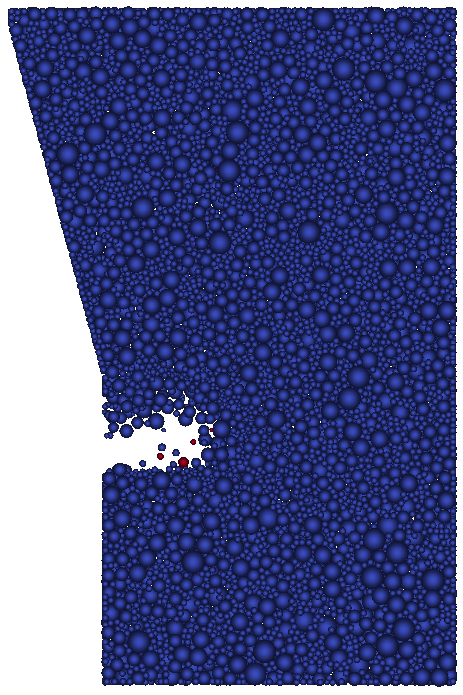
\includegraphics[width=.21\columnwidth]{images/296ver_slice_4mslf}
	  \label{fig:296ver_slice_4mslf}
  }
  \quad
    \subfloat[\acs{mus} = 0.1, $u_{lim}$ = 0.1 m/s]
    {
	  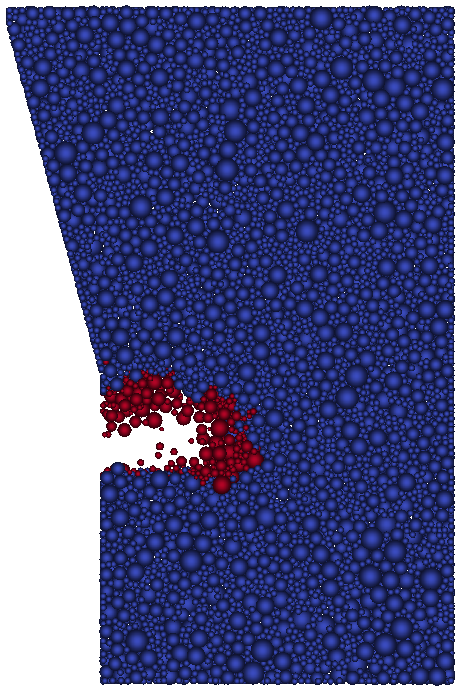
\includegraphics[width=.21\columnwidth]{images/295ver_slice_01mslf}
	  \label{fig:295ver_slice_01mslf}
  }
  \quad
    \subfloat[\acs{mus} = 0.1, $u_{lim}$ = 0.01 m/s]
    {
	  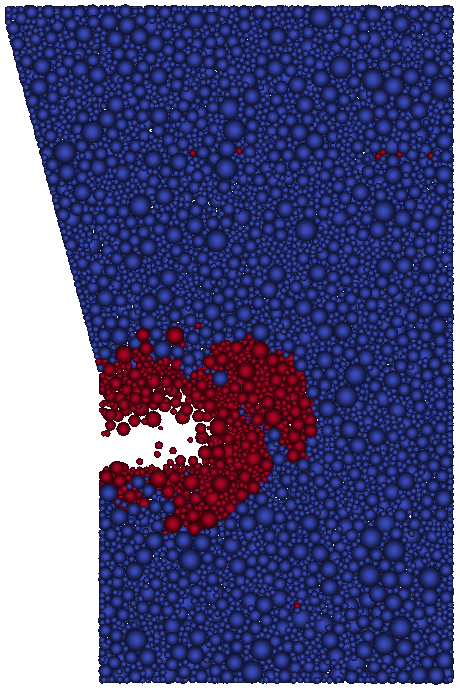
\includegraphics[width=.21\columnwidth]{images/294ver_slice_001mslf}
	  \label{fig:294ver_slice_001mslf}
  }
  \quad
  \subfloat[\acs{mus} = 0.1, $u_{lim}$ = 0.003 m/s]
  {
	  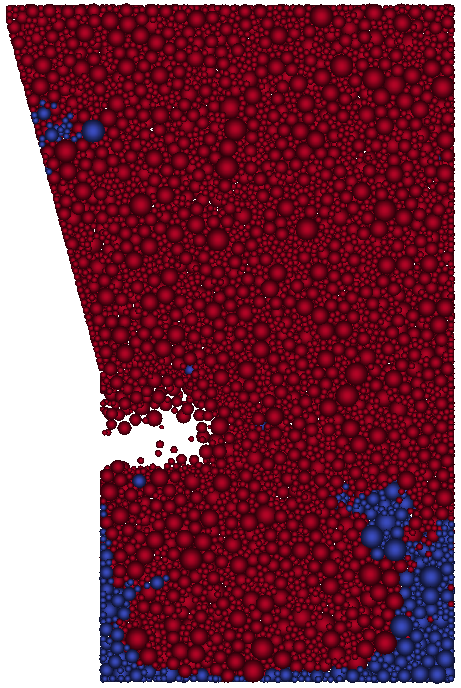
\includegraphics[width=.21\columnwidth]{images/293ver_slice_0003mslf}
	  \label{fig:293ver_slice_0003mslf}
  }
  \\
  \subfloat[\acs{mus} = 0.9, $u_{lim}$ = 4 m/s]
  {
	  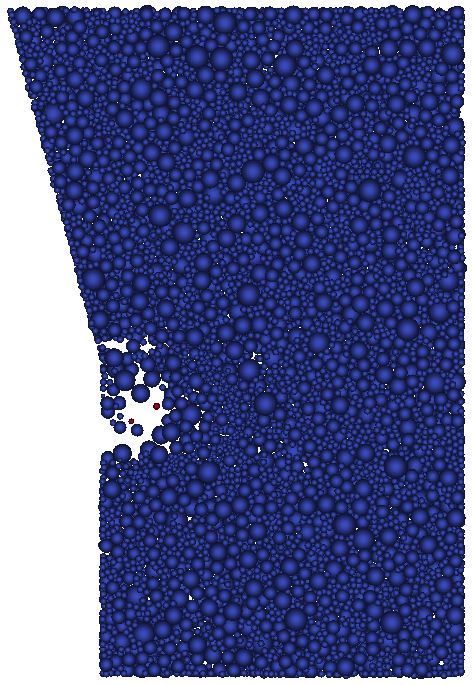
\includegraphics[width=.21\columnwidth]{images/266ver_slice_4mshf}
	  \label{fig:266ver_slice_4mshf}
  }
  \quad
    \subfloat[\acs{mus} = 0.9, $u_{lim}$ = 0.1 m/s]
    {
	  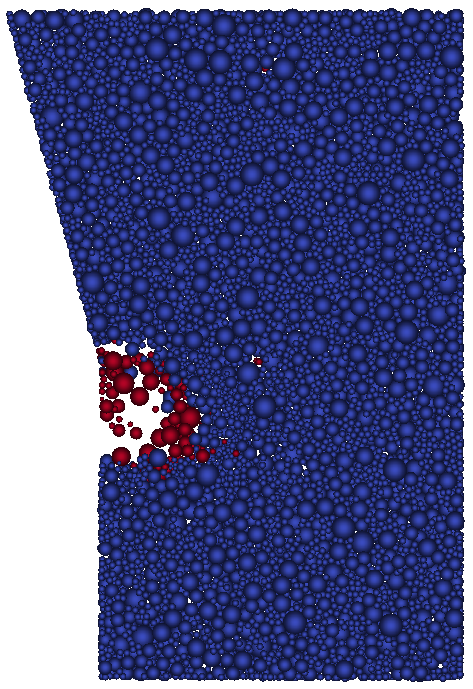
\includegraphics[width=.21\columnwidth]{images/267ver_slice_01mshf}
	  \label{fig:267ver_slice_01mshf}
  }
  \quad
    \subfloat[\acs{mus} = 0.9, $u_{lim}$ = 0.01 m/s]
    {
	  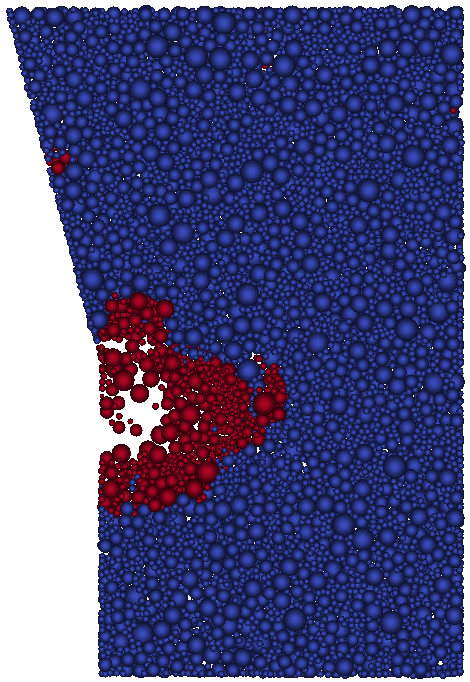
\includegraphics[width=.21\columnwidth]{images/268ver_slice_001mshf}
	  \label{fig:268ver_slice_001mshf}
  }
  \quad
  \subfloat[\acs{mus} = 0.9, $u_{lim}$ = 0.003 m/s]
  {
	  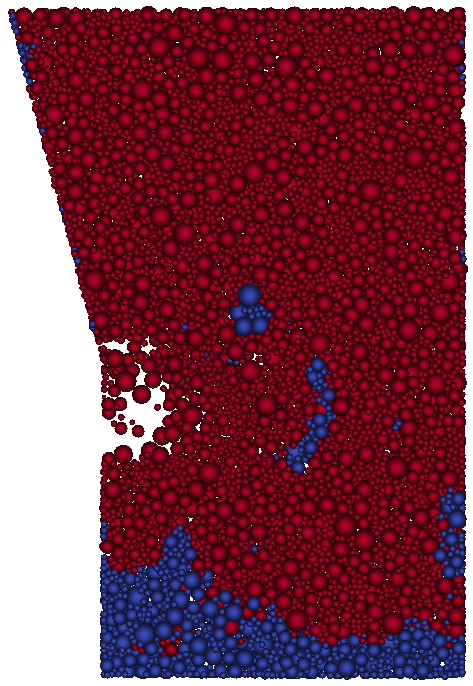
\includegraphics[width=.21\columnwidth]{images/269ver_slice_0003mshf}
	  \label{fig:269ver_slice_0003mshf}
  }
  \\  
  \caption[Vertical slice of particle velocity 2]{Vertical slice of particle
  velocity 2. Red particles are faster than the $u_{lim}$. The effect of sliding
  friction over the particle velocity is consistent. Many more particles show
  faster velocity than the threshold in every representation.}
  \label{fig:298verticalslicelf}
\end{figure}